%% =====================================================================
%%  4_empirical_study.tex --- Chapter 4: Empirical Study
%% =====================================================================

\chapter{Empirical Study} \label{chap:empirical}

This chapter situates the artefact of Chapter~\ref{chap:method} in its industrial context and assembles the empirical material on which Chapter~\ref{chap:results} reports. It opens with a short profile of the partner organisation, walks the AS-IS process and the 8 pain points it surfaces, and sketches the TO-BE artefact that follows from those pain points. The bulk of the chapter then specifies the evaluation design: the data sources, the 3 block composition of the evaluation set, the supplier level failure clustering, the per-case ground truth on the buyer sample, the synthetic perturbation matrix and the ground truth construction protocol. The chapter's contribution is twofold: it specifies the case in which the artefact is evaluated, with explicit operational measures, and it constructs an evaluation set under which the next chapter's results are interpreted.


%% -----------------------------------------------------------------
\section{Introduction}
\label{sec:emp:intro}

This chapter operationalises the Chapter~\ref{chap:method} methodology against a real procurement case at Hilti AG. The case scope is fixed throughout: the Procurement function inside Hilti's Sourcing, Innovation and Competence Division; the commerce eXtensible Markup Language (cXML) Advanced Shipping Notice (ASN) as the validated document; and the rule register introduced in Section~\ref{sec:method:taxonomy}.


%% -----------------------------------------------------------------
\section{Case organisation: Hilti and the procurement function}
\label{sec:emp:case}

The empirical work reported here is conducted inside Hilti AG, a Liechtenstein headquartered manufacturer of professional construction, fastening and measuring equipment, with a 2025 global turnover of CHF 6.3~bn, around 34{,}400 employees and a direct sales footprint in more than 120 countries.\footnote{Company figures from Hilti Group public reporting.} Specifically, the work is conducted inside the Sourcing, Innovation and Competence Division, where a Procurement department is responsible for the source-to-pay transactions that govern incoming goods from external suppliers. The case is methodologically informative in 3 respects: a defined gate at which the artefact intervenes (the partner’s enterprise system), a documented operational process and a buyer validated pain-point inventory (Section~\ref{sec:emp:asis}), and a heterogeneous supplier profiles base across different integration modes, against which the artefact's supplier conditioned layer can be exercised. Following the case study guidance of \citet{yin2018case} and \citet{runeson2009}, this study treats the case as suited to single case industrial study on 3 grounds: a clearly defined unit of analysis, a stable operational context, and a researcher accessible site that permits both archival data extraction and stakeholder interviews.

The Advanced Shipping Notice (ASN) is at the centre of the case. An ASN is the cXML document that a supplier transmits to Hilti, through the procurement platform's electronic data interchange (EDI) channel, to declare the contents and the dispatch parameters of an outbound shipment against a previously issued Purchase Order (PO). On receipt, the ASN is matched against the PO baseline by the partner's enterprise system; a mismatch, whether in quantity, unit of measure, currency, delivery date or any of numerous further attributes, blocks the goods receipt, and the buyer is drawn into a manual reconciliation loop that involves reading the cXML by hand and emailing the supplier.


Table~\ref{tab:emp:asis_baseline} consolidates the operational baseline of the AS-IS process. The volume figures describe the function; the per-defect handling time and the time to resolution are reported by the buyer team, drawn from interviews with 3 analysts and past ASN resolution logs. Production ASN defects are usually cleared in a single iteration, whereas pre-integration cases run longer because they involve repeated back-and-forth with the supplier. The annual cost projection that scales these figures, with its assumptions, is derived in Appendix~\ref{app:operational}.

\begin{table}[htbp]
\centering
\caption{AS-IS operational baseline.}
\label{tab:emp:asis_baseline}
\small
\begin{tabular}{@{}lp{7.5cm}@{}}
\toprule
\textbf{Metric} & \textbf{Value} \\
\midrule
Live function volume & Of the order of 28,000 ASNs per year \\
Manual handling per defect          & 30 to 90 minutes (buyer reported) \\
Time to resolution, production      & 2 to 5 days, usually a single iteration\\
Time to resolution, pre-integration & About 2 months on average (9 cases sampled from past resolution email threads, ranging from days to roughly 5 months)\\
\bottomrule
\end{tabular}
\end{table}


%% -----------------------------------------------------------------
\section{The AS-IS process and its pain points}
\label{sec:emp:asis}

The AS-IS ASN validation process is a swimlane covering 4 actors: the Hilti buyer, the partner's system, the supplier, and the communication channel; the swimlane is shown in Figure~\ref{fig:emp:asis}, and is reproduced with the pain point markers annotated in Appendix~\ref{app:emp:asis} (Figure~\ref{fig:app:asis}). The process unfolds in 5 phases. Phase~1 (PO Creation) is internal to Hilti. Phase~2 (ASN Submission) is the supplier transmitting the cXML to the partner system. Phase~3 (Decision) is binary: the partner system either accepts the ASN or rejects it without further triage. Phase~4 is the manual remediation loop: the buyer checks the errors flagged by the partner system, fixes the ASN by hand, and exchanges emails with the supplier until both sides agree on a corrected version. Phase~5 closes the case with the Transport Advice creation.

\begin{figure}[htbp]
\centering
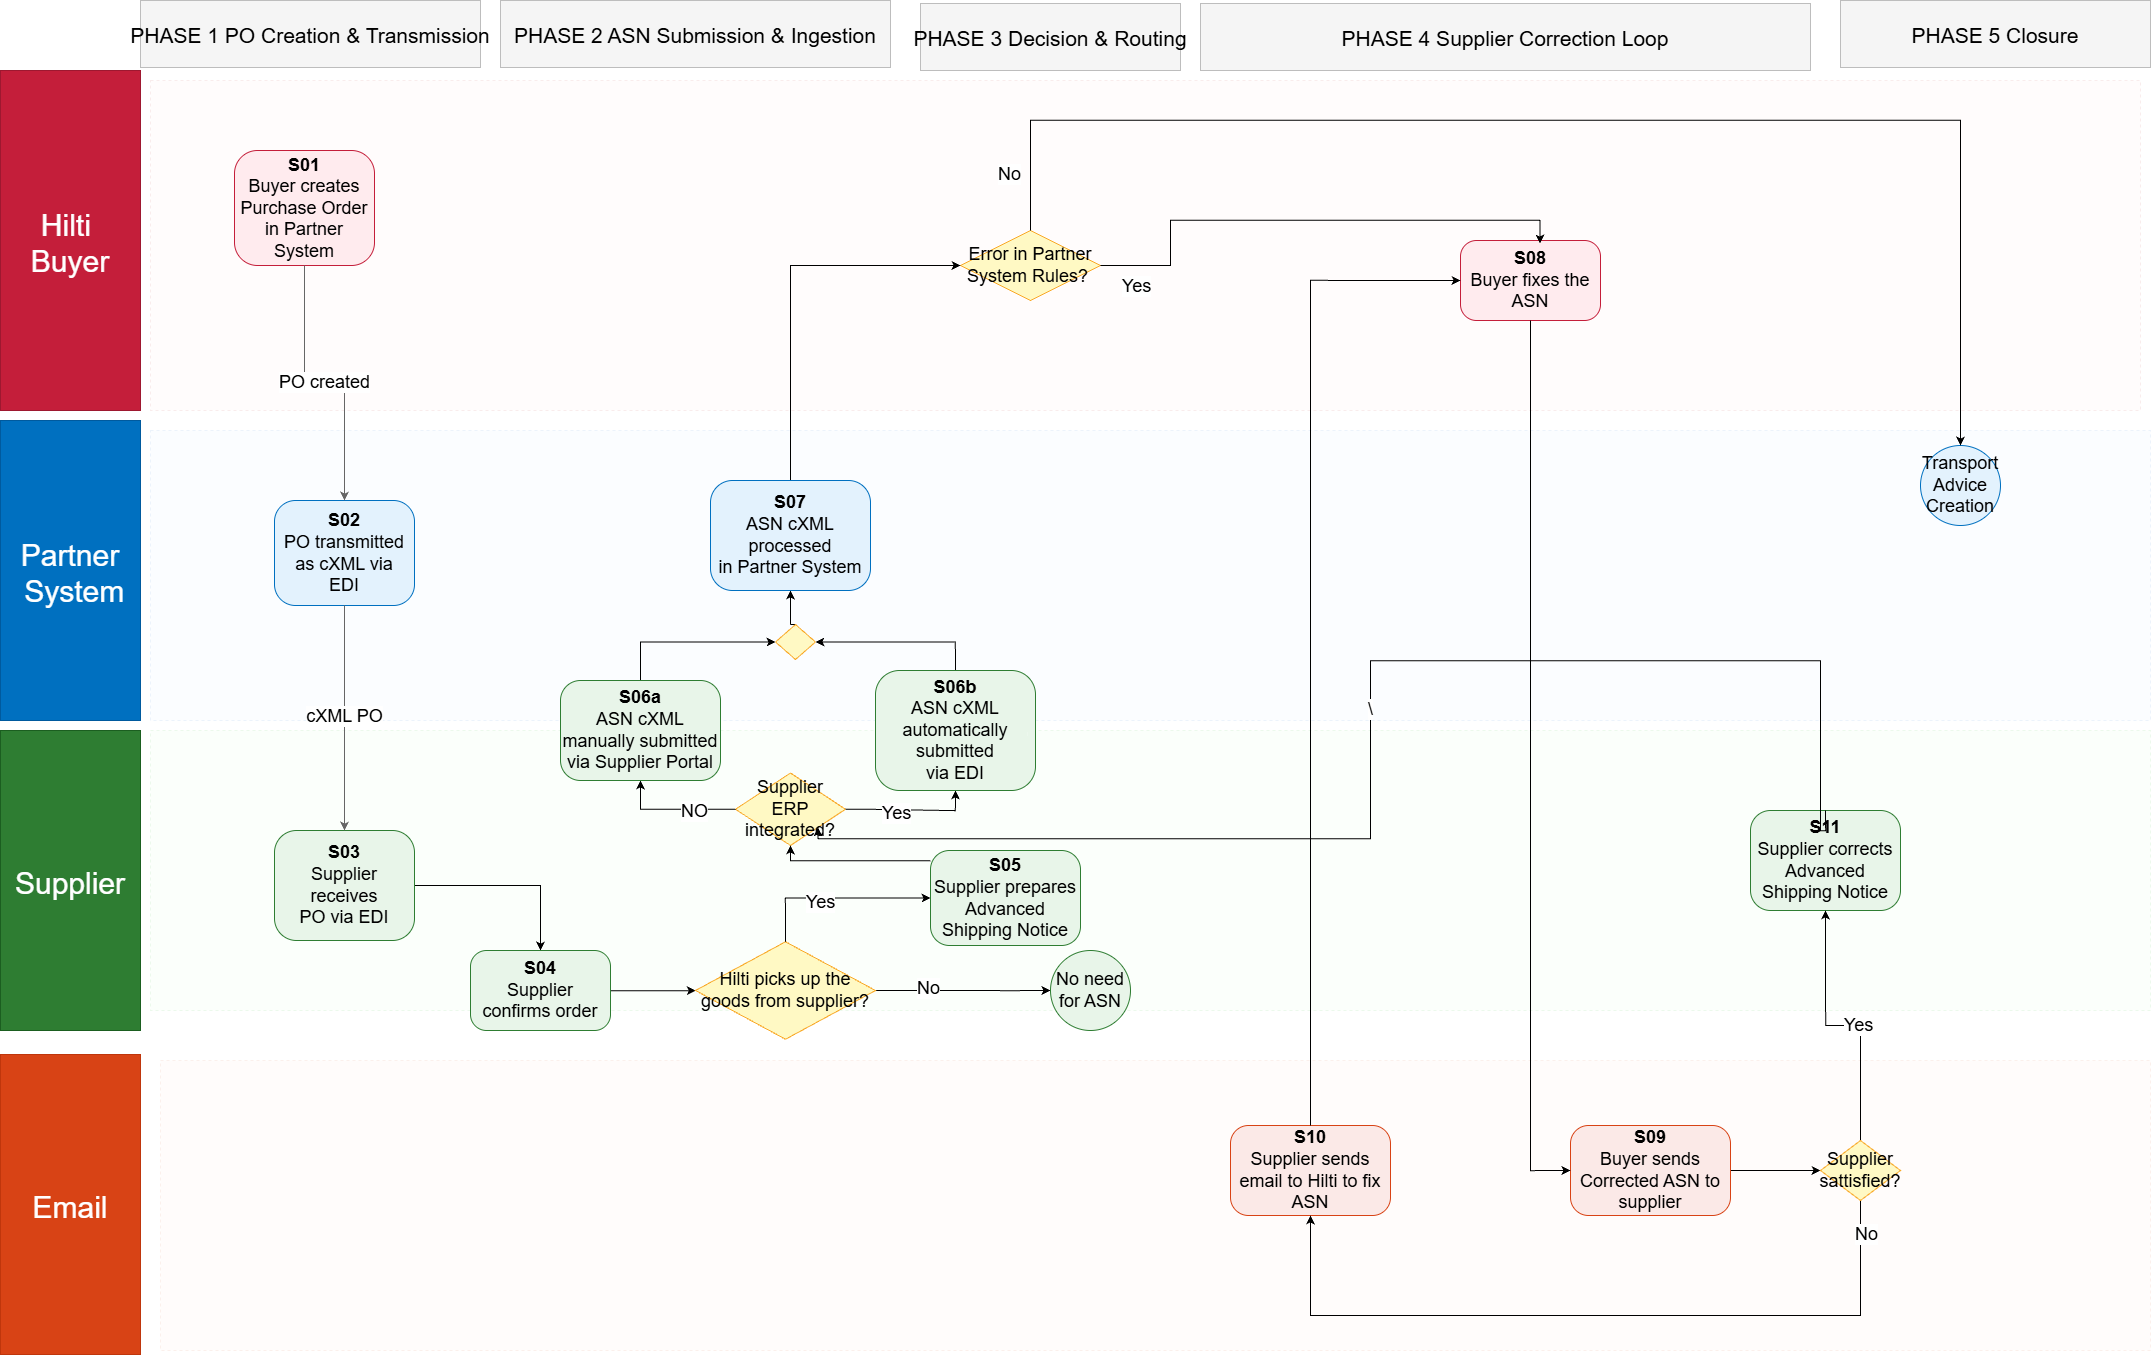
\includegraphics[width=\textwidth]{Figures/fig_4_1_asis_swimlane.pdf.png}
\caption{AS-IS PO--ASN validation process.}
\label{fig:emp:asis}
\end{figure}

The pain point annotation was produced jointly with the buyer team. The 8 pain points it surfaces are reproduced in Table~\ref{tab:emp:painpoints}, with severity assigned by the buyer team on a 3 level scale (Critical, High, Medium) and a root cause attached to each.

\begin{table}[htbp]
\centering
\caption{AS-IS pain points, with severity and root cause.}
\label{tab:emp:painpoints}
\footnotesize
\begin{adjustbox}{max width=\textwidth}
\begin{tabular}{@{}llp{1.6cm}p{9.5cm}@{}}
\toprule
\textbf{\#} & \textbf{Pain point} & \textbf{Severity} & \textbf{Root cause} \\
\midrule
P1 & No automated content validation & Critical & Static field checks only; no semantic, cross-document or supplier history validation, and some defects fail silently. \\
P2 & Manual correction loop & Critical & Buyers interpret each ASN error by hand, email the supplier, and iterate until a corrected version is agreed; the per-defect time and round trip latency are buyer reported rather than measured in this study. \\
P3 & Manual portal entry & High & Light account suppliers type ASNs by hand into the procurement portal, producing typographic and unit of measure errors. \\
P4 & Faulty ERP integration mapping & High & Misconfigured cXML-to-ERP mappings produce the same defect on every ASN from a specific supplier. \\
P5 & No tracking visibility & High & No central tracker; buyers cannot see which ASNs are pending, stuck or escalated. \\
P6 & No supplier history & Medium & Recurring defects are not retained per supplier; the same mistakes recur until solved. \\
P7 & Binary disposition & High & Only accept or reject; no review state for minor or recoverable discrepancies, for example, a late delivery (R03) is rejected on the same gate as a wrong currency (R08), despite the first being recoverable in negotiation. \\
P8 & No audit trail & Medium & Corrections scattered across email; no structured log of why each ASN was accepted or rejected. \\
\bottomrule
\end{tabular}
\end{adjustbox}
\end{table}

For P1, the partner system applies only schema validation and a closed list of static field checks at receipt; it performs no semantic or cross-document check, and some of those checks fail silently, dropping the ASN without an error to the buyer. The full mapping of what the static checks cover, rule by rule, is in Appendix~\ref{app:emp:coverage}.

The 8 pain points fall into 3 classes: upstream, processing and audit. The artefact does not address all 8; it prioritises by severity and targets. The upstream class (P1, P4) is met by the content validation pipeline, which runs the full rule register on every ASN. The processing class (P2, P7) is met by the tiered disposition layer, which adds a REVIEW state between accept and reject, a design informed by the broader human-in-the-loop principles of \citet{amershi2019}. The audit class (P6, P8) is met by the supplier conditioned prompting layer of Section~\ref{sec:method:supplier} and by a structured audit log of every input, prediction and disposition. P3 (manual portal entry) is organisational, not technical, and is out of scope by design; P5 (tracking visibility) is left to future work.

These 3 classes recur in Section~\ref{sec:emp:groundtruth} when the rule level evidence is read against the partner's static check coverage.


%% -----------------------------------------------------------------
\section{The TO-BE artefact}
\label{sec:emp:tobe}

The TO-BE swimlane is shown in Appendix~\ref{app:emp:asis} (Figure~\ref{fig:emp:tobe}). The TO-BE adds 3 new actors to the AS-IS picture: a cloud host that runs the deterministic parser, the prompt builder and the enforcer; a language model service that normalises the cXML payload and assesses each rule against the PO baseline; and a SharePoint log that persists every input, every prediction and every disposition, addressing P8.

The pipeline progresses through 6 phases. Phase~1 (PO Creation and Transmission) is unchanged from the AS-IS. Phase~2 (ASN Submission and Ingestion) captures each cXML envelope into the inbound records; the partner system's existing static checks still fire here but are now one input among many rather than the gatekeeper. Phase~3 (AI Processing) is the new core and realises stages 2 to 6 of the Section~\ref{sec:method:pipeline} pipeline: the deterministic parser ingests the cXML, the language model normalises it into structured JSON, the prompt builder assembles the rule register R01--R22, the PO baseline and the supplier history of Section~\ref{sec:emp:clustering} into a single prompt, the language model assesses each rule and emits a per rule verdict with severity and evidence, and the enforcer reduces those verdicts to a master report. Phase~4 (Decision and Routing) collapses the master report to one of 3 dispositions: PASS, REVIEW or REJECT; addressing pain point P7; REVIEW cases are routed to the buyer for adjudication, REJECT cases trigger an auto-generated correction request that is sent only with the buyer's sanction; the pipeline never communicates with the supplier without a buyer in the loop. Phase~5 (Supplier Correction Loop) closes the case once the buyer has dispatched the discrepancy list and the resubmitted ASN triggers the Transport Advice creation (Phase~6, Closure) that ends the original workflow.

The artefact is therefore human-in-the-loop by design rather than as a fallback, a positioning that builds on the human-in-the-loop work of \citet{amershi2019} and \citet{bansal2021}. The buyer's role shifts from the AS-IS pattern of full manual reconciliation to a review pattern in which the pipeline produces the per rule verdicts, the rationale and the draft correspondence, and the buyer adjudicates REVIEW cases, sanctions REJECT requests before dispatch, and handles the edge cases the pipeline cannot decide. The audit log records the buyer's overrides alongside the pipeline's verdicts, providing a structured source of disagreement data that can inform subsequent revisions to the prompt template and the rule register. The supplier conditioning layer of Section~\ref{sec:method:supplier} draws on the same source: each supplier's prior failure record is built from the audit log entries the buyer has validated, so the history the model reads is grounded in confirmed dispositions and is refreshed as the buyer reviews new cases.

The pipeline is evaluated under the 5 designs specified in Section~\ref{sec:method:ablation} (pure LLM, post hoc, LLM-as-judge, in generation and pre hoc), and the validation logic is the 7 stage compound pipeline of Section~\ref{sec:method:pipeline}. The TO-BE adds the cloud host, the language model service and the SharePoint log, but the stage sequence is unchanged.


%% -----------------------------------------------------------------
\section{Evaluation design}
\label{sec:emp:eval}

This section specifies the conditions under which Chapter~\ref{chap:results} evaluates the artefact: where the data come from and how the evaluation set is composed across 3 blocks (Section~\ref{sec:emp:sources}), which protocol produced the buyer labels (Section~\ref{sec:emp:protocol}), how supplier level failures cluster in the prior corpus that feeds the supplier conditioned prompting layer (Section~\ref{sec:emp:clustering}), what the buyer validated ground truth on the buyer sample looks like (Section~\ref{sec:emp:groundtruth}) and how the synthetic perturbation matrix completes per rule coverage (Section~\ref{sec:emp:synthetic}).


%% -----------------------------------------------------------------
\subsection{Data sources and inclusion}
\label{sec:emp:sources}

The evaluation admits 3 sources: the production stream, the pre-integration stream and a synthetic set; no other source is admitted. A case enters the evaluation set only when

(i)~the source system holds its cXML, guarding the completeness of the document of record,

(ii)~the matching purchase order is also in the source system, guarding referential integrity against the order baseline, and

(iii)~its disposition has been buyer validated or is known by construction, guarding ground truth provenance.

The evaluation set is the residue of a 3 stage filter that implements the inclusion rule (Figure~\ref{fig:emp:filter}) and it contains 100~ASNs across 3 blocks by source: production (Block~A, 28~ASNs), pre-integration (Block~B, 4~ASNs) and synthetic (Block~C, 68~ASNs). The synthetic block carries dispositions known by construction. One case, S-18 (duplicate detection, rule R18), is checked by re-submission rather than a static edit, so 67 of the 68 are evaluable as static dispositions. The production and pre-integration blocks carry the buyer validated dispositions of Section~\ref{sec:emp:protocol}. The full block summary, with each block's source, case range, structural shape and disposition mix, is in Appendix~\ref{app:emp:supporting} (Table~\ref{tab:emp:blocks}).

\begin{figure}[htbp]
\centering
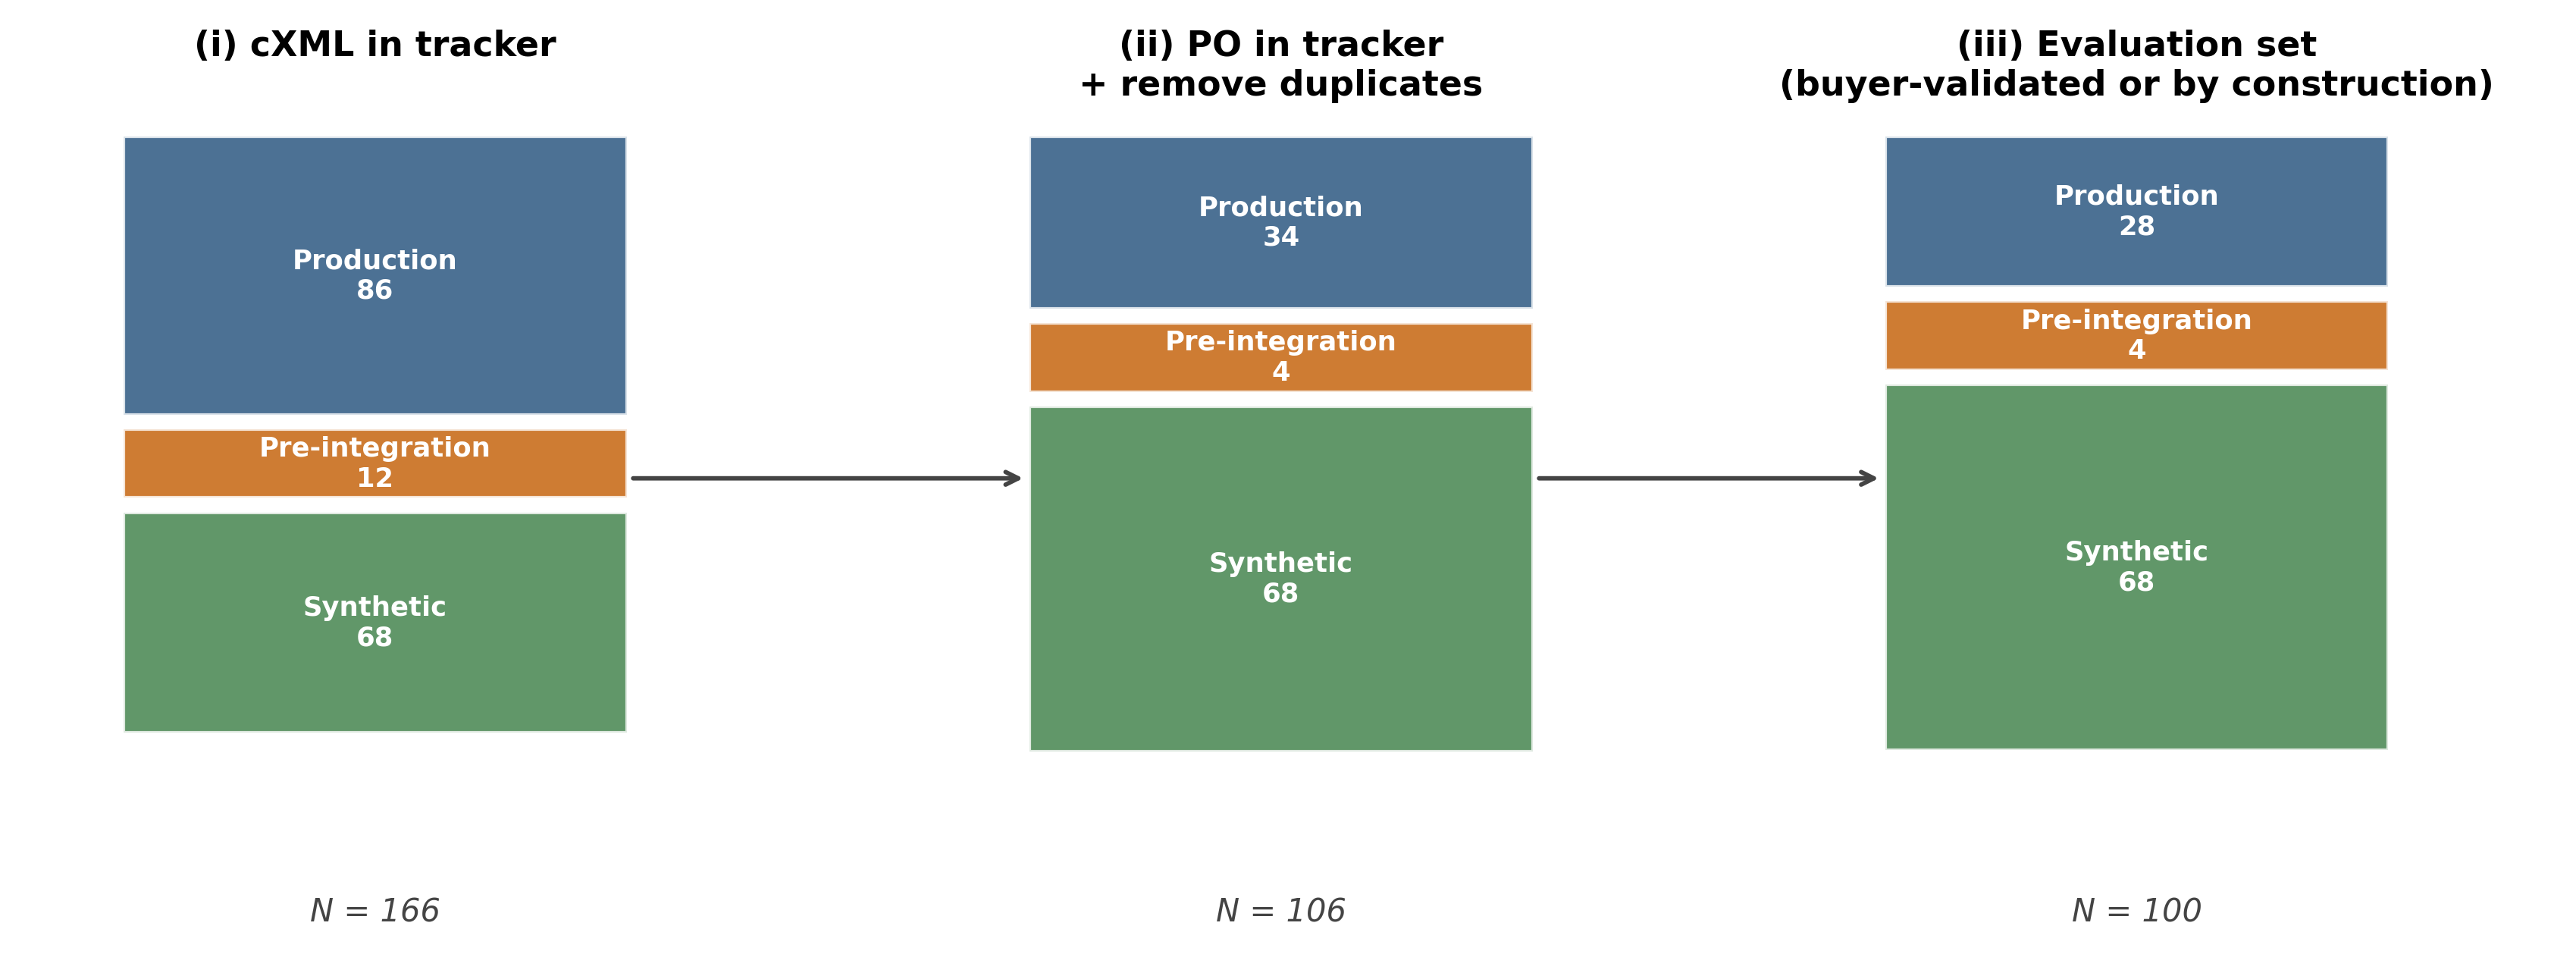
\includegraphics[width=\textwidth]{Figures/fig_4_6_dataset_flow.png}
\caption{Dataset assembly funnel from the raw scrape to the 100-case evaluation set.}
\label{fig:emp:filter}
\end{figure}

\paragraph{Production stream.} The production stream is extracted from the partner's platform tracker, which logs delivery and notification events for source-to-pay traffic. Both rejected and accepted ASNs are eligible, provided the cXML and the matching purchase order are still in the tracker, so the block deliberately mixes the two; the split is reported in Section~\ref{sec:emp:groundtruth}.

\paragraph{Pre-integration stream.} The pre-integration stream comes from the same tracker but covers supplier onboarding, where document exchange with a new supplier is tested before live traffic begins; these cases were curated by the buyer team in a dedicated session. Both real world streams share one constraint: the tracker retains only the last 30 days, which caps how many cases any single scrape yields.

\paragraph{Synthetic perturbation.} The real world cases are too few to exercise every rule individually, so synthetic cases close the gap. Each is a clean production ASN altered by deliberate edits to the cXML, generated deterministically from schema anchored templates rather than by a language model. The block holds 51 single rule mutants (S-01 to S-51) and 17 multi-rule scenarios (SYN-M01 to SYN-M17); their design, and the expected dispositions that follow directly from the edits, are detailed in Section~\ref{sec:emp:synthetic}, so no buyer review is needed.


%% -----------------------------------------------------------------
\subsection{Ground truth construction protocol}
\label{sec:emp:protocol}

The labelling protocol described below was defined in collaboration with the same buyer team that produced the AS-IS swimlane and the pain-point table of Section~\ref{sec:emp:asis}, and applies to every real world ASN that enters the evaluation set. The protocol is deliberately blind: the analysts do not see the pipeline's prediction, and the cases are interleaved on the worksheet by source rather than by the pipeline's verdict, so the analysts are not nudged towards a disposition.

The buyer ground truth is a consensus of 3 procurement analysts. Each labelled every case independently under the blind protocol, and the verdicts were reconciled: agreements stood, and disagreements were adjudicated in a short joint review to a single agreed disposition and rule list. To stay within the analysts' limited availability only this consensus was retained, so an inter-rater coefficient cannot be computed retrospectively. A consensus of several experts is taken here as a stronger reference than a single annotator, drawing on the multi-annotator agreement literature of \citet{artstein2008} and \citet{fleiss1971}. Each label also carries a 5 point analyst confidence, reported in Section~\ref{sec:emp:groundtruth}. The panel is small and shares the partner organisation's conventions, so the reference reflects one organisation's reading of the rules; recording the per analyst labels and widening the panel is part of the deferred validation discussed in Chapter~\ref{chap:results}.

The checklist, the 2 rules pre-filled N/A, and the annotation interface are described in Appendix~\ref{app:emp:annotation}.


%% -----------------------------------------------------------------
\subsection{Failure clustering by supplier}
\label{sec:emp:clustering}

The pipeline (Section~\ref{sec:method:supplier}) feeds the language model a short history of each supplier's past failures, taken from the evaluation set itself. Of the 19 distinct suppliers in the evaluation set, 5 have at least 2 buyer validated cases; the other 14 contribute no history and stay in the evaluation set only as cases.

\begin{table}[htbp]
\centering
\caption{Supplier prior corpus, grouped by failure archetype.}
\label{tab:emp:suppliers}
\footnotesize
\begin{adjustbox}{max width=\textwidth}
\begin{tabular}{@{}lllll p{6cm}@{}}
\toprule
\textbf{Archetype} & \textbf{Supplier} & \textbf{Country} & \textbf{n} & \textbf{Disposition mix} & \textbf{Notes} \\
\midrule
Strongest historical signal       & S1  & AT & 9 & 9 REJECT  & Recurring transport, address, packaging, mandatory field and unit price defects \\
Recurring buyer flagged defects   & S2  & CH & 2 & 2 REJECT  & Unit price and currency mismatch with transport/address drift \\
Upstream bug false positives      & S3  & CH & 3 & 3 PASS    & Timezone issue; content clean \\
Upstream bug with packaging gap   & S4  & CN & 2 & 2 REVIEW  & Timestamp artefact plus missing packaging dimensions; surfaced as R21 REVIEW \\
Onboarding REVIEW pattern         & S12 & CZ & 2 & 2 REVIEW  & Cross-PO setup with delivery date and packaging gaps \\
\bottomrule
\end{tabular}
\end{adjustbox}
\par\vspace{0.2em}\footnotesize{Supplier labels are non-contiguous because the corpus is a subset of the full supplier inventory.}
\end{table}

Each supplier's history shows up as one sentence in the system prompt; the 5 sentences exactly as the model reads them are reproduced in Appendix~\ref{app:emp:supporting} (Table~\ref{tab:emp:prompts}).


The corpus shows 2 patterns. It is heavy tailed: S1 alone contributes 9 of the 18 prior ASNs and every REJECT. And a few rules recur across suppliers (Appendix~\ref{app:emp:supporting}, Table~\ref{tab:app:perrule}), so the artefact must catch them independently of supplier history. The corpus covers 5 of the 19 real world suppliers and is refreshed from buyer dispositions in production.

The corpus above is drawn from the real world sample. The synthetic block (Block~C) is built independently, and part of it is run with the supplier history switched on, switched off, and replaced by a placebo (a different supplier's facts under the same label); this supports the supplier conditioning ablation of Section~\ref{sec:method:supplier}.


%% -----------------------------------------------------------------
\subsection{Ground truth on the real world sample}
\label{sec:emp:groundtruth}

Under the labelling protocol of Section~\ref{sec:emp:protocol}, the buyer validated ground truth covers the 28 production cases of Block~A and the 4 pre-integration cases of Block~B at the disposition and rule levels; the synthetic block (Block~C) carries dispositions known by construction and is reported in Section~\ref{sec:emp:synthetic} instead. Table~\ref{tab:emp:gtsummary} reports the supporting summary statistics. The per-case detail underlying both is in Appendix~\ref{app:emp:supporting} (Table~\ref{tab:app:percase}).

\begin{table}[htbp]
\centering
\caption{Real world ground-truth summary.}
\label{tab:emp:gtsummary}
\footnotesize
\begin{adjustbox}{max width=\textwidth}
\begin{tabular}{@{}lp{9.5cm}@{}}
\toprule
\textbf{Metric} & \textbf{Value} \\
\midrule
Cases                                            & 32 \\
Distinct suppliers                               & 19 \\
Buyer dispositions                               & 4 PASS, 15 REVIEW, 13 REJECT \\
Cases with at least one buyer-flagged rule       & 28 of 32 (88\,\%) \\
Mean rules per flagged case                      & 3.8 (range 1--7) \\
Top 3 rules                                      & R14 (24 cases), R13 (21), R21 (18) \\
Rule classes covered                             & PO baseline (4 rules), packaging (3 rules), delivery-date (1 rule), unit of measure (1 rule) \\
Analyst confidence (1--5)                        & Mean 4.2; 16 cases at 5, 5 at 4, 11 at 3; none below 3 \\
\bottomrule
\end{tabular}
\end{adjustbox}
\end{table}
The summary supports a few readings. Most cases are buyer flagged on at least one rule, and the few PASS cases come from suppliers S3 and S6, whose visible failures trace to an upstream timestamp artefact rather than a content defect. Flagging concentrates on a handful of suppliers and on the PO baseline and packaging rule classes, which the partner's static checks do not cover (Appendix~\ref{app:emp:coverage}). The pre-integration cases carry buyer validated dispositions and enter Chapter~\ref{chap:results} on the same footing as the production cases, and the labels carry high analyst confidence.


%% -----------------------------------------------------------------
\subsection{Synthetic perturbation matrix}
\label{sec:emp:synthetic}

Each mutant is a clean production ASN modified by a deterministic, schema-anchored edit, a quantity change, a date shift, a removed packaging element, and so on, and the expected disposition follows directly from the edit through the disposition rule of Section~\ref{sec:method:disposition}. The generator is deterministic rather than language model based. The single rule mutants follow the property based testing tradition \citep{bartocci2023} and the multi-rule scenarios the higher order mutation tradition \citep{wang2022hom, wu2025hom}. Rules R11 and R22 receive N/A on every mutant, by construction and as in the labelling protocol: R11 (schema compliance) is an ingestion check that every schema-valid mutant passes before rule evaluation, and R22 (order fulfilment) needs cumulative quantities across earlier ASNs that a single static mutant cannot provide. This is expected and holds for every mutant.

The block contains 51 single rule mutants (S-01 to S-51) and 17 multi-rule scenarios (SYN-M01 to SYN-M17). All are built on 4 base supplier templates, so each rule is tested against more than one formatting profile. The first 22 single rule mutants each target one rule, covering the whole register R01 to R22. The remaining single rule mutants add 3 groups: boundary cases that sit just on a rule's pass or fail threshold, cases that break the same rule in different ways or by different amounts, and cases that repeat a defect across different supplier templates. The multi-rule scenarios each combine 2 or 3 edits on a single ASN. Some cases are \emph{PASS controls}, clean cases that should pass. The PASS controls let the block measure both whether the pipeline catches real defects (sensitivity) and whether it leaves clean ASNs alone (specificity), and they reduce the tendency of synthetic cases to be easier than human authored ones \citep{gill2025synthetic}. The full per-case inventory is in Appendix~\ref{app:emp:supporting} (Tables~\ref{tab:app:mutants_full} and~\ref{tab:app:multirule}).


The matrix exercises each active rule at least once and balances the 2 rule regimes; the per rule coverage is detailed in Appendix~\ref{app:emp:supporting}.


%% -----------------------------------------------------------------
\section{Chapter conclusion}
\label{sec:emp:conclusion}

This chapter set the conditions under which the artefact is evaluated. The AS-IS process was documented and decomposed into 8 pain points, and the artefact positioned as the TO-BE insertion of the validation pipeline between ASN submission and the partner's static check. The evaluation set holds 100~ASNs: 28~production, 4~pre-integration and 68~synthetic, assembled under a uniform inclusion rule. The supplier prior corpus carries 5 suppliers and 18 prior ASNs under a leakage-preventing $n_{\text{prior}} \geq 2$ rule. The buyer ground truth covers all 32 buyer cases, the 28 production and 4 pre-integration cases, and flags all but 4 of them on at least one rule, concentrated on classes the partner's static checks do not cover; the synthetic block covers every rule by construction. The next chapter exercises the pipeline across this set under the 5 designs and reports the results.
